\scanpage{64}

\margin{(\unsure{$k$ anneau comm.})}
Mais si $F$\inserted{sur $X_*$}\inserted{(un $k$-Module)} est loc. constant, alors on vérifie facilement que
\[
C^*(X_*,F)\simeq
\Gamma\bigl(X_*,\underbrace{(C_*^*|X_*)}_{C_{X_*}^*}\otimes_{k_*}F\bigr)
\]
\margin{\figure{\begin{tikzpicture}
\node[draw,ellipse,align=left] {$\unsure{\text{NB on pose}}$\\$C_*^*=C_*^*k\quad\unsure{\text{pour abréger}}$};
\end{tikzpicture}}}

et on vérifie tout de suite que $C_{X_*}^*\otimes_{k_*}F$ est une résolution de $F$, laquelle est d'ailleurs \uline{flasque}. \deleted{\unsure{Donc}} (que $F$ soit loc. constant ou non, d'ailleurs). Donc, sans hypothèse de loc. constance sur $F$, $C^*(X_*,F)$ permet de calculer la coh. de $X_*$ à coeff. dans $F$ (i.e. \unsure{on a} un isom. can.
\margin{\figure{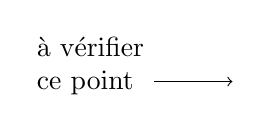
\begin{tikzpicture}
\node[align=left,anchor=east] at (0,0) {à vérifier\\ce point};
\draw[->] (0,-.2)--(1,-.2);
\end{tikzpicture}}}
\[
H^*\left(
\underbrace{C^*(X_*,F)}_{
\substack{\Vert\,\mathrm{dfn}\\\Gamma(X_*,C_{X_*}^*\otimes_kF)}
}
\right)\simeq H^*(X_*,F)
\]
\unsure{Isom.} \deleted{\unsure{compatible}} fonctoriel en $F$ (et même en $(X_*,F)\ldots$) et compatible avec les hom. cobords. De même pour le calcul de l'hypercohomologie de $X_*$ à coeff. ds un complexe de $k$-Modules $F^*$. En termes de catégories dérivées, on aura un isomorphisme de foncteurs triangulés
\[
R\Gamma(X_*,F^*)\simeq
\underbrace{C^*(X_*,F^*)}_{
\substack{\text{pour degré total}\\
\text{associé aux}\\
\text{deux degrés}\\
(\unsure{\text{proven. de }C\text{ et de}}\\F^*)}}
\]
\margin{\figure{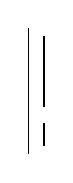
\begin{tikzpicture}
\draw (0,0)--(0,1.6);
\draw (.2,.6)--(.2,1.5);
\draw (.2,.1)--(.2,.4);
\end{tikzpicture}}}
\margin{63}
